\appendix
\section{Supplementary benchmark visualizations}\label{app:benchmark_visualizations}

This appendix provides supplementary descriptive views of the locked-test results and computational effort. Unless otherwise stated, cell summaries and plotted points use the three common seeds. The performance--cost figure uses summed recorded fit times for cache-miss candidates; it excludes cache hits and is not end-to-end wall-clock search time.

Figures~\ref{fig:heatmap_mccf1_mcc_test} and~\ref{fig:heatmap_accuracy_accuracy_test} provide cell-level views of the protocol-aligned locked-test metric across backbone and optimizer. Their purpose is to expose interactions that are compressed in the optimizer-level table, not to add a new statistical test.

\begin{figure}[!htbp]\centering
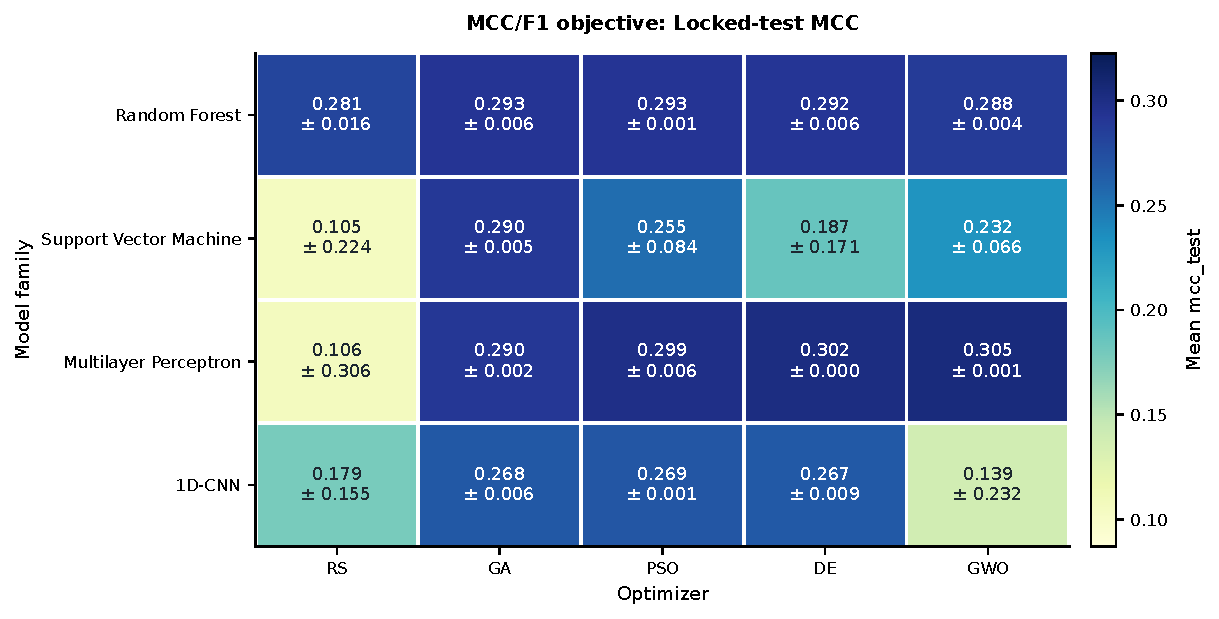
\includegraphics[width=0.96\linewidth]{figures/heatmap_mccf1_mcc_test.pdf}
\caption{Locked-test MCC by classifier backbone and optimizer after selection under the MCC/$F_1$ validation objective. Each cell reports the mean and standard deviation across the three common seeds; color encodes the mean.}
\label{fig:heatmap_mccf1_mcc_test}\end{figure}

\begin{figure}[!htbp]\centering
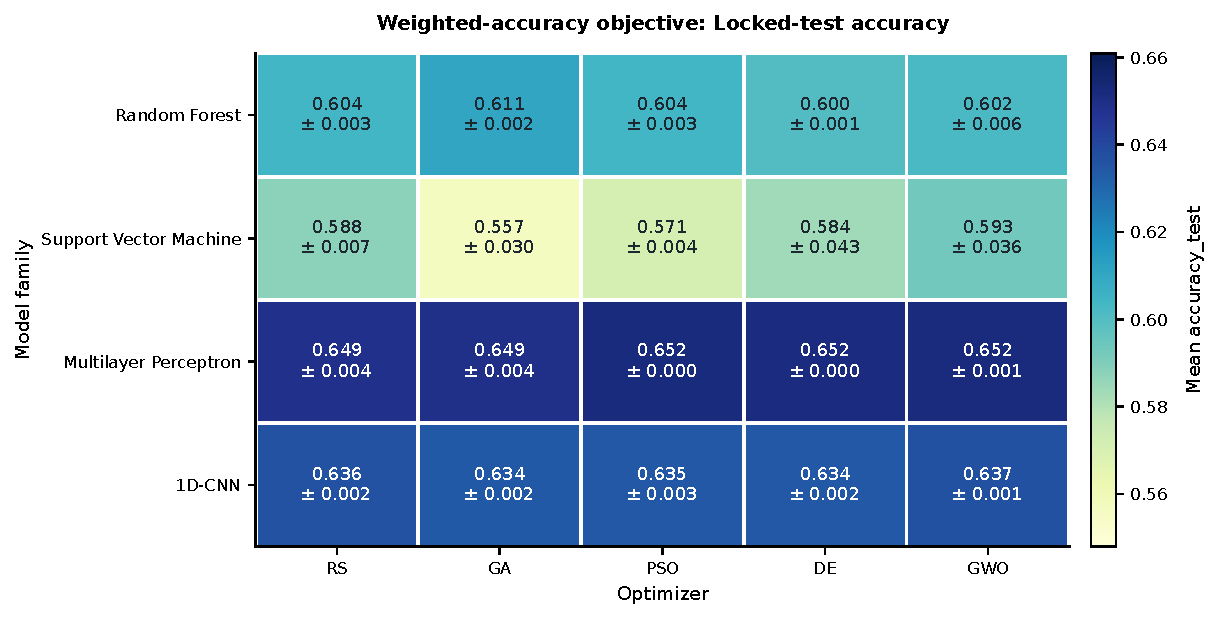
\includegraphics[width=0.96\linewidth]{figures/heatmap_accuracy_accuracy_test.pdf}
\caption{Locked-test accuracy by classifier backbone and optimizer after selection under the weighted-accuracy validation objective. Each cell reports the mean and standard deviation across the three common seeds; color encodes the mean.}
\label{fig:heatmap_accuracy_accuracy_test}\end{figure}
\FloatBarrier

Across the heatmaps, RF is comparatively uniform across optimizers under MCC/$F_1$, while SVM, MLP, and 1D-CNN show more optimizer-dependent MCC patterns. Under weighted-accuracy selection, MLP forms the strongest and most consistent row; 1D-CNN is competitive but remains below it, while SVM shows wider optimizer variation. These cell patterns agree with Table~\ref{tab:optimizer_primary_metrics}: no optimizer preserves the same relative position for every backbone and protocol. Because each cell averages only three seeds, the colors are descriptive and should be read alongside the displayed dispersion.

Figure~\ref{fig:test_mcc_seed_boxplots} shows how much seed-level MCC variation is hidden by the cell means, while Figure~\ref{fig:optimizer_average_ranks} summarizes optimizer ordering across the 12 matched backbone--seed blocks. The two views address complementary questions: dispersion within model--optimizer cells and variation in optimizer rank across backbones.

\begin{figure}[!htbp]\centering
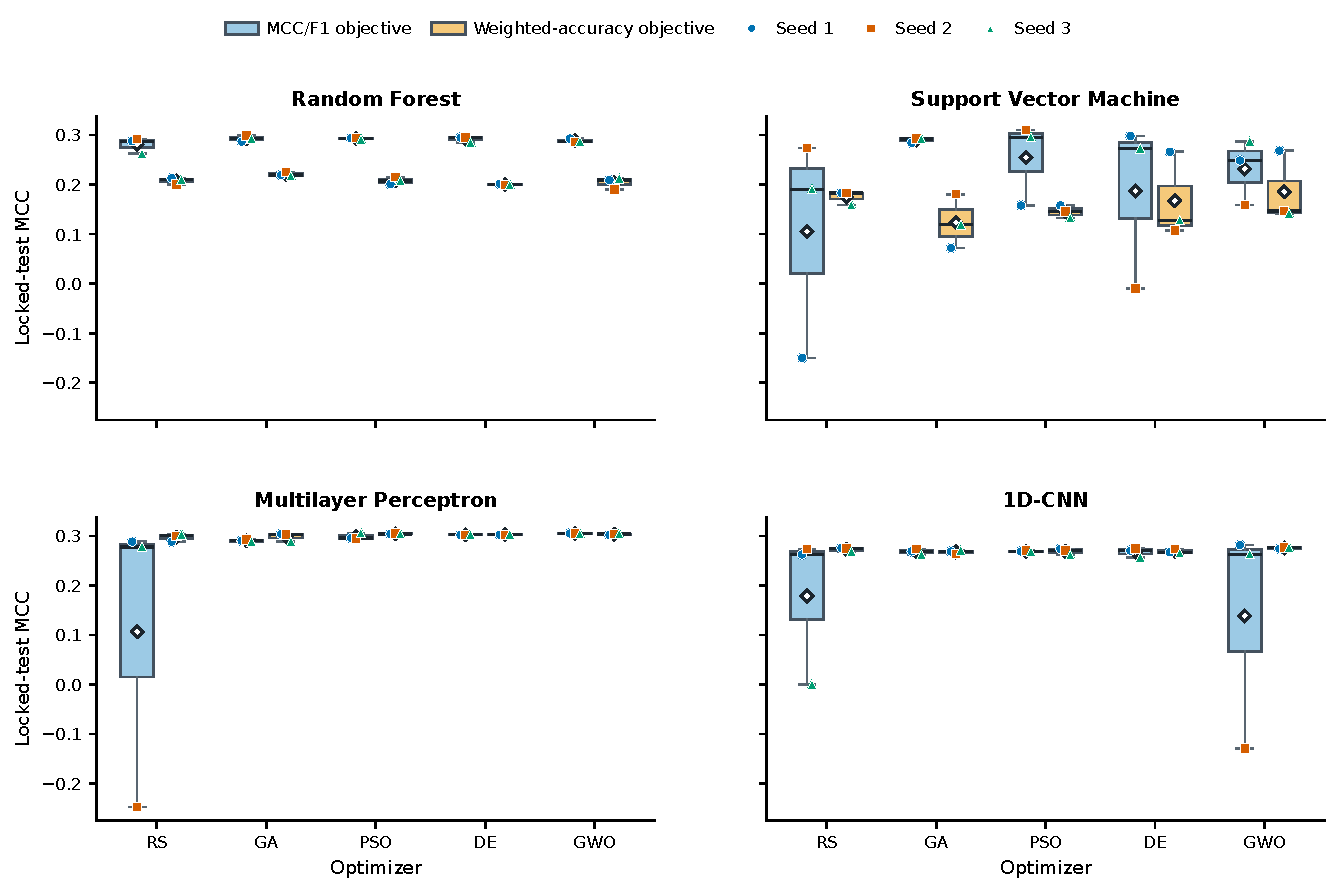
\includegraphics[width=0.98\linewidth]{figures/test_mcc_seed_boxplots.pdf}
\caption{Locked-test MCC across optimizer--seed outcomes for each backbone under both validation objectives. Boxes summarize the three common seeds, individual markers show seed-level values, and diamonds mark the mean. The small number of seeds makes these descriptive displays rather than inferential evidence.}
\label{fig:test_mcc_seed_boxplots}\end{figure}

\begin{figure}[!htbp]\centering
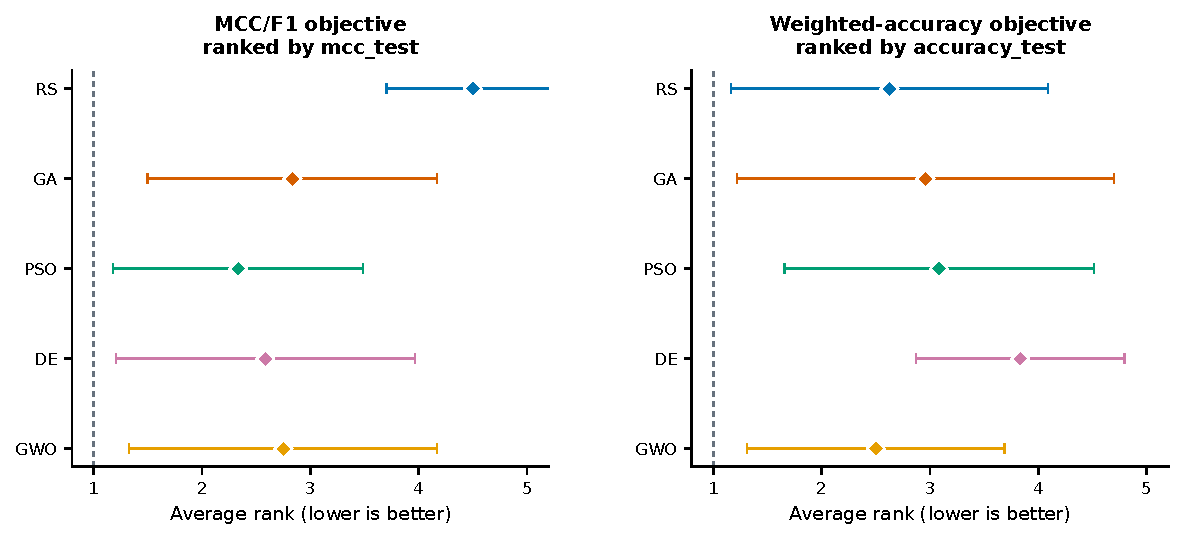
\includegraphics[width=0.96\linewidth]{figures/optimizer_average_ranks.pdf}
\caption{Descriptive average ranks of the five optimizers across 12 matched backbone--seed blocks (four backbones and three common seeds). Rankings use locked-test MCC under the MCC/$F_1$ protocol and locked-test accuracy under the weighted-accuracy protocol. Error bars denote one standard deviation of block-level ranks; lower average rank is better. No significance test is implied by this visualization.}
\label{fig:optimizer_average_ranks}\end{figure}

The boxplots show tight RF seed clusters but visibly broader MCC variation for SVM and for selected MLP and 1D-CNN optimizer cells, including Random Search. This supports the dispersion reported in Table~\ref{tab:predictive_summary} and cautions against reading a three-seed mean as a stable cell-level estimate. The optimizer-rank plot changes its central ordering between protocols and has substantial block-level spread; it is therefore a descriptive check on heterogeneity, not an optimizer significance test or a universal league table.

Figure~\ref{fig:performance_vs_fit_time} places predictive score against recorded candidate-fit effort, and Figure~\ref{fig:benchmark_radar} gives a normalized overview of predictive and computational dimensions. The former helps identify score--effort trade-offs across backbone--optimizer combinations; the latter is included only as a compact visual summary because normalization obscures the original units.

\begin{figure}[!htbp]\centering
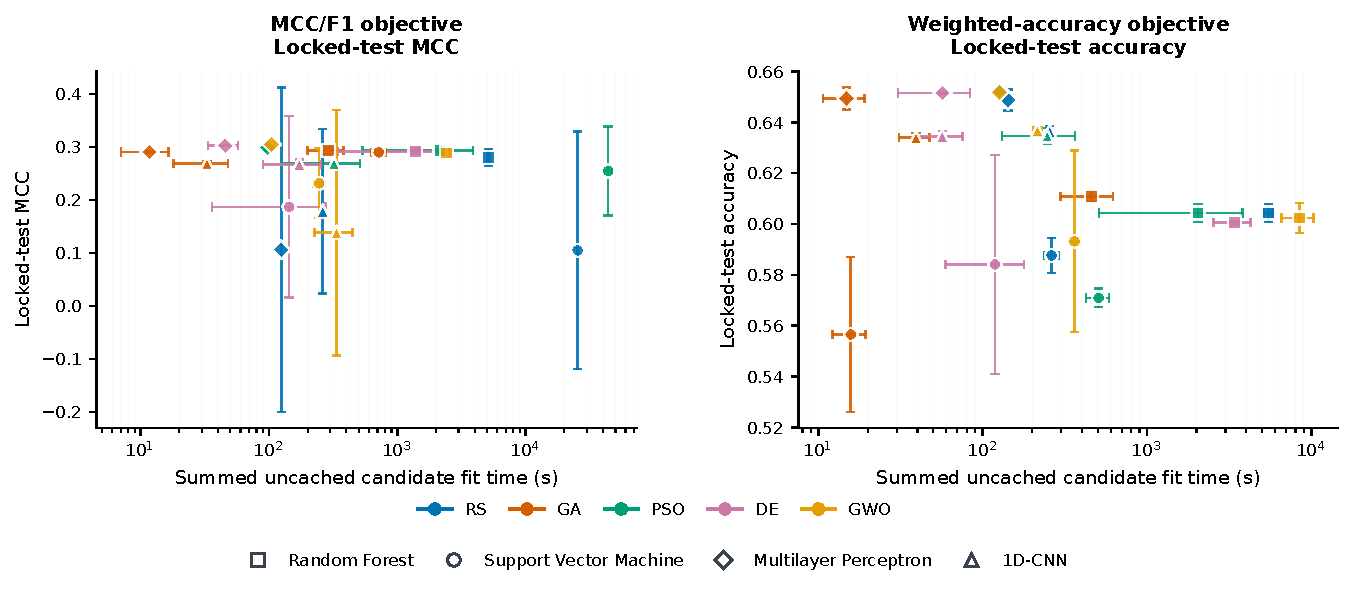
\includegraphics[width=0.98\linewidth]{figures/performance_vs_candidate_fit_time.pdf}
\caption{Locked-test performance versus summed model-fit time for cache-miss candidate evaluations. The left panel uses test MCC for the MCC/$F_1$ protocol and the right panel uses test accuracy for the weighted-accuracy protocol. Point color identifies the optimizer and marker shape identifies the backbone; points show means and error bars show one standard deviation across the three common seeds. The horizontal axis is cumulative recorded fit time, not end-to-end wall-clock search time.}
\label{fig:performance_vs_fit_time}\end{figure}

\begin{figure}[!htbp]\centering
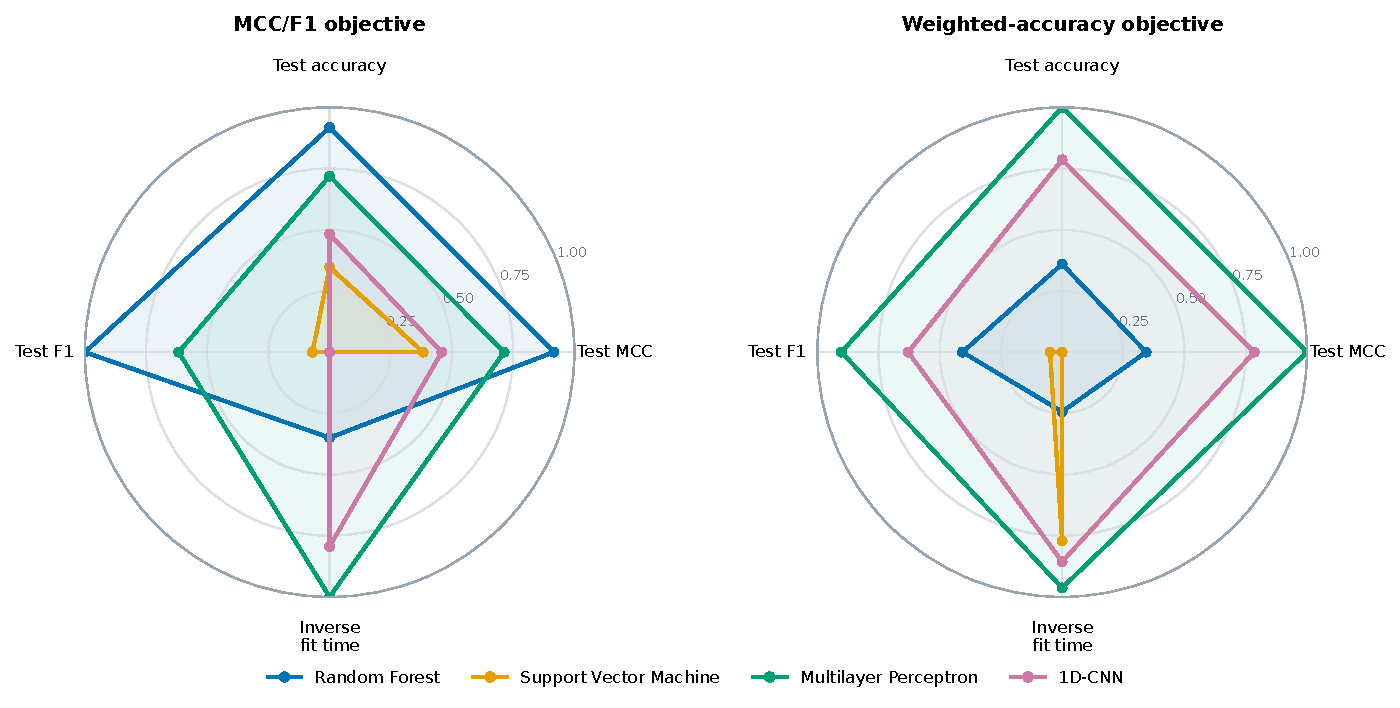
\includegraphics[width=0.98\linewidth]{figures/radar_overview_normalized.pdf}
\caption{Complementary radar summary of test MCC, test accuracy, test $F_1$, and inverse candidate-fit time by backbone under each validation objective. Values are min--max normalized across the eight backbone--protocol averages; higher values indicate better results on each axis. Candidate-fit time is log-transformed before inversion and normalization.}
\label{fig:benchmark_radar}\end{figure}
\FloatBarrier

The combinations in Figure~\ref{fig:performance_vs_fit_time} occupy different performance--effort positions, so the apparent advantage depends on whether predictive score or candidate-fit effort is prioritized. Its horizontal coordinate is summed uncached fit time and must not be interpreted as total optimizer wall-clock cost. In Figure~\ref{fig:benchmark_radar}, the profile shapes also change across protocols and metrics, reinforcing that no one scalar summary represents all outcomes. The normalized radar is consequently complementary only; quantitative comparisons should use the original-scale results in the main tables.
